\subsection{Physically Based Rendering}

In einer 3D-Szene eines Videospiels will man natürlich komplexere Objekte als Primitives darstellen. Diese Objekte bestehen aus vielen Primitives. Die Primitives in diesem Falle sind meist Dreiecke. 
Die Art der Zusammensetzung ist unterschiedlich: manchmal kann es effizienter sein aneinander hängende Dreiecke zu verwenden, jedoch werden meistens nur einzelne Dreiecke gerendert. 
Einige Programme verwenden auch andere Polygone, welche aber auch aus Dreiecken bestehen. Daher ist dies Irrelevant. 
Ein Objekt, gebildet aus Dreiecken, nennt man \textit{Mesh}. Als Beispiel ist das Mesh eines Delfins in \cref{Dolphin} dargestellt. Die Farbe bzw. die "`Haut"' eines Objektes wird aus einem zweidimensionalem Bild gelesen, genannt wird dies eine \textit{Textur}. 
Dafür besitzt jeder Vertex zusätzlich zu seiner Position eine zweidimensionale Position auf der Textur. So kann ermittelt werden, welche Pixel der Textur verwendet werden sollen.
Mit Mesh und Textur ist es möglich ein Objekt in einer dreidimensionalen Szene anzuzeigen, doch würde dies in einem Videospiel nicht überzeugen. Hier wird \ac{PBR} verwendet. \ac{PBR} ist eine Möglichkeit eine realistischere dreidimensionale Szene zu erzeugen in dem physikalische Phänomene wie Licht berücksichtigt werden. 
Wie ein Objekt auf Licht reagiert, hängt von verschiedenen Größen ab, wie die eigentliche Farbe des Objekts, die Oberflächenstruktur, aber auch die Farbe und Richtung des einfallenden Lichts. Alle Eigenschaften eines Objekts die sich auf die Farbe auswirken werden in einem \textit{Material} zusammengefasst. 
Ein Objekt, welches gerendert werden soll besitzt beides: ein \textit{Mesh} und ein \textit{Material}, was zusammengefasst \textit{Model} genannt wird.

Es gibt zwei Arten von Lichtquellen in der FM3D-Engine: \textit{Directional Light} und \textit{Point Lights}. Eins Directional Light besitzt, eine Richtung aber \underline{keine} Position. Diese Art kann verwendet werden um zum Beispiel eine Sonne zu simulieren. Diese ist soweit von der Erde entfernt, dass die Position irrelevant ist. Die Richtung hingegen ist wichtig und von der Tageszeit abhängig. 

Point Lights sind das genaue Gegenteil. Sie besitzen keine Lichtrichtung sondern scheinen in alle Richtungen gleich, dafür besitzten sie aber eine genau festgelegte Position, welche relevant ist, da die Lichtstärke mit zunehmendem Abstand kleiner wird. Point Lights können verwendet werden, um die meisten Lichtquellen darzustellen: Als Beispiel nehme man Laternen oder Fackeln. 
Man kann aber nicht nur zwischen Lichtquellen unterscheiden sondern auch zwischen verschiedenen Arten des ausgesendeten Lichts. Die FM3D-Engine verwendet ein Lichtmodell genannt "Ambient/Diffuse/Specular". \textit{Ambient Light} ist das Licht welches man jeden Tag sieht, auch wenn gerade keine Sonne scheint oder man sich nicht in direkter Nähe einer Lichtquelle befindet. Es entsteht dadurch, dass Licht von allen Objekten wieder teilweise reflektiert wird und so eine schwache und gleichmäßige Beleuchtung entsteht. Ohne diese wäre es hinter einem Haus, welches die Sonne verdeckt, komplett finster. 
Die zweite Lichtart ist \textit{Diffuse Light}, welches abhängig von dem Auftrittswinkel des Lichtstrahls ist. Die dem Licht zugewandte Seite eines Würfels heller ist als die nur teilweise zugewandte Seite und die abgewandte Seite erfährt gar kein \textit{Diffuse Light}. \textit{Specular light} modelliert die Lichtstrahlen, welche von einem Objekt reflektiert und in die Linse der Kamera bzw. in die Augen des Betrachters gelangen. Dies wird als blendendes, helles Licht wahrgenommen und ist oft auf metallischen Obeflächen zu erkennen. Diese drei Lichtarten sind in \cref{Img:Lights} dargestellt.

Alle Lichtberechnungen müssen für jeden Pixel ausgeführt werden und laufen daher im Fragment shader ab.
Um die Farbe eines gerenderten Pixels zu bestimmen benötigt man einige Informationen: Die Position, die Farbe, den Normalenvektor und Specular factor des Pixels. Diese 4 Informationen reichen für alle Lichtberechnungen aus. Die Phase in der sie erstellt bzw. berechnet werden ist unterschiedlich. Ein Teil wird außerhalb des Programms in externen Programmen erstellt und als Vertex im Mesh oder als Information im Material. Dabei kann man unterscheiden zwischen:
\begin{itemize}
	\item Der Information, die sich zwischen verschiedenen Objekten unterscheidet, aber nicht innerhalb des Objekts
	\item Information die für jeden Vertex anders ist aber für jeden Pixel nur linear interpoliert werden muss
	\item Information die für jeden Pixel anders ist
\end{itemize}
Ersteres ist das simpelste und kann einfach im Material gespeichert werden, da jedes Objekt ein eigenes Material haben kann und es anders als ein Mesh nicht viel Speicher benötigt. 
Die Vertexinformationen werden im \ac{VBO} des Mesh gespeichert und automatisch linear interpoliert, wenn sie an den Fragment-Shader weiter gegeben werden. Pixelinformationen müssen einzeln in einer Textur gespeichert werden, diese ist dann im Material enthalten, wobei sie nur referenziert wird, damit verschiedene Materials die gleichen Texturen verwenden können. In den Vertexinformationen müssen hierfür zusätzlich Texturkoordinaten gespeichert werden. Daraus ergeben sich die folgenden Werte:

\begin{table}
	\caption{Vertex Aufbau}
	\label{table:VertexAufbau}
	\centering
	\begin{tabular}{lll}\toprule[1.5pt]
		Datentyp & Name & Beschreibung \\\midrule
		3D-Vektor & Position & Position des Vertex \\
		2D-Vektor & Textur Koordinate & Position des Vertex auf der Textur \\
		3D-Vektor & Normal & Normalenvektor zum Dreieck \\
		32-Bit Farbe & Color & Farbe des Vertex (optional, Standard ist weiß) \\
		3D-Vektor & Tangent & Tangentenvektor des Dreiecks. Benötigt wenn \\
		 & & Normal maps verwendet werden. Siehe \cref{section:Normalmapping}\\\bottomrule[1.5pt]
	\end{tabular}
\end{table}
\begin{table}
	\caption{Material Aufbau}
	\centering
	\begin{tabular}{lll}\toprule[1.5pt]
	Datentyp & Name & Beschreibung \\\midrule
	32-Bit Farbe & Color & Farbe des gesamten Objekts \\
	Textur & Color Texture & Gibt die Farbe jedes Pixels des Objektes an \\
	Textur & Normal map & Gibt den Normalenvektor jedes Pixels an. \\
	 & & Genaueres in \cref{section:Normalmapping} \\
	Float & Specular factor & Faktor für das resultierende Specular light \\
	Textur & Specular map & Specular factor für jeden Pixel. Der Faktor \\
	 & & des ganzen Objekts wird weiterhin verwendet \\
	 Boolean & UseWireframe & Gibt an ob ganze Dreiecke gerendert werden sollen\\
	  & & oder nur die Kanten. (Nützlich für Debugging)\\\bottomrule[1.5pt]
\end{tabular}
\end{table}


\begin{figure}
	\begin{center}
		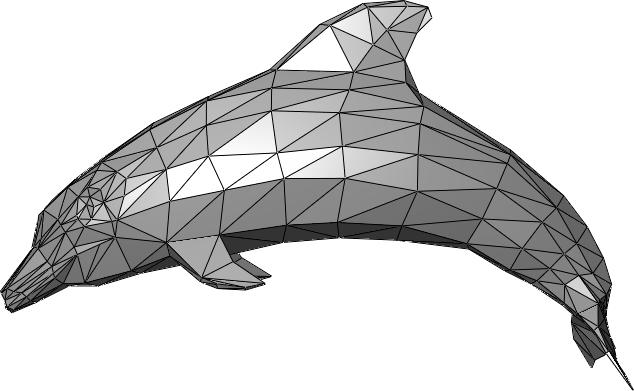
\includegraphics[width=0.5\textwidth]{06anhang/bilder/delphin.jpg}
		\caption{Mesh eines Delfins}
		\label{Dolphin}
	\end{center}
\end{figure}
\begin{figure}
	\centering
	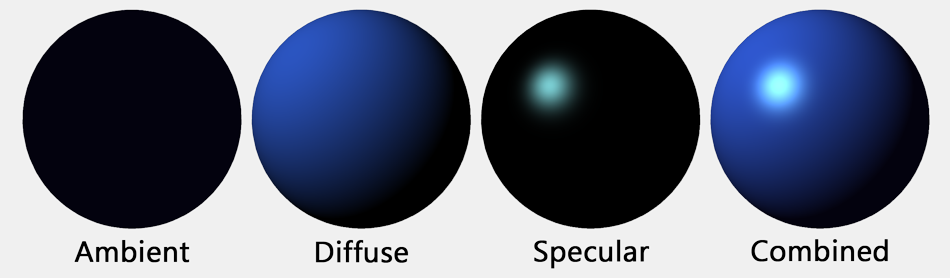
\includegraphics[scale=0.4]{02theorie/amb_diff_spec.png}
		
	Quelle: https://clara.io/img/pub/amb\textunderscore diff\textunderscore spec.png
	\caption{Lights}\label{Img:Lights}
\end{figure}

Die FM3D-Engine verwendet \textit{Deferred Rendering}. Dies bedeutet, dass erst alle Objekte einer Szene gerendert und die Ergebnisse daraus in mehreren Buffern gespeichert werden. Danach wird für jede Lichtquelle ein weiterer Renderprozess ausgeführt, wobei die vorher genannten Buffer als Input dienen. Das Ergebnis ist dann die zu sehende \cref{Img:Lights}. Der Vorteil hierbei ist, dass keine Lichtberechnungen unnötig ausgeführt werden, da alle Pixel später zusehen sind und es keine Begrenzung für die Anzahl der Lichtquellen gibt. 